\section{Durchführung}
\label{sec:Durchführung}

\subsection{Versuchsaufbau}

\begin{figure}
\centering
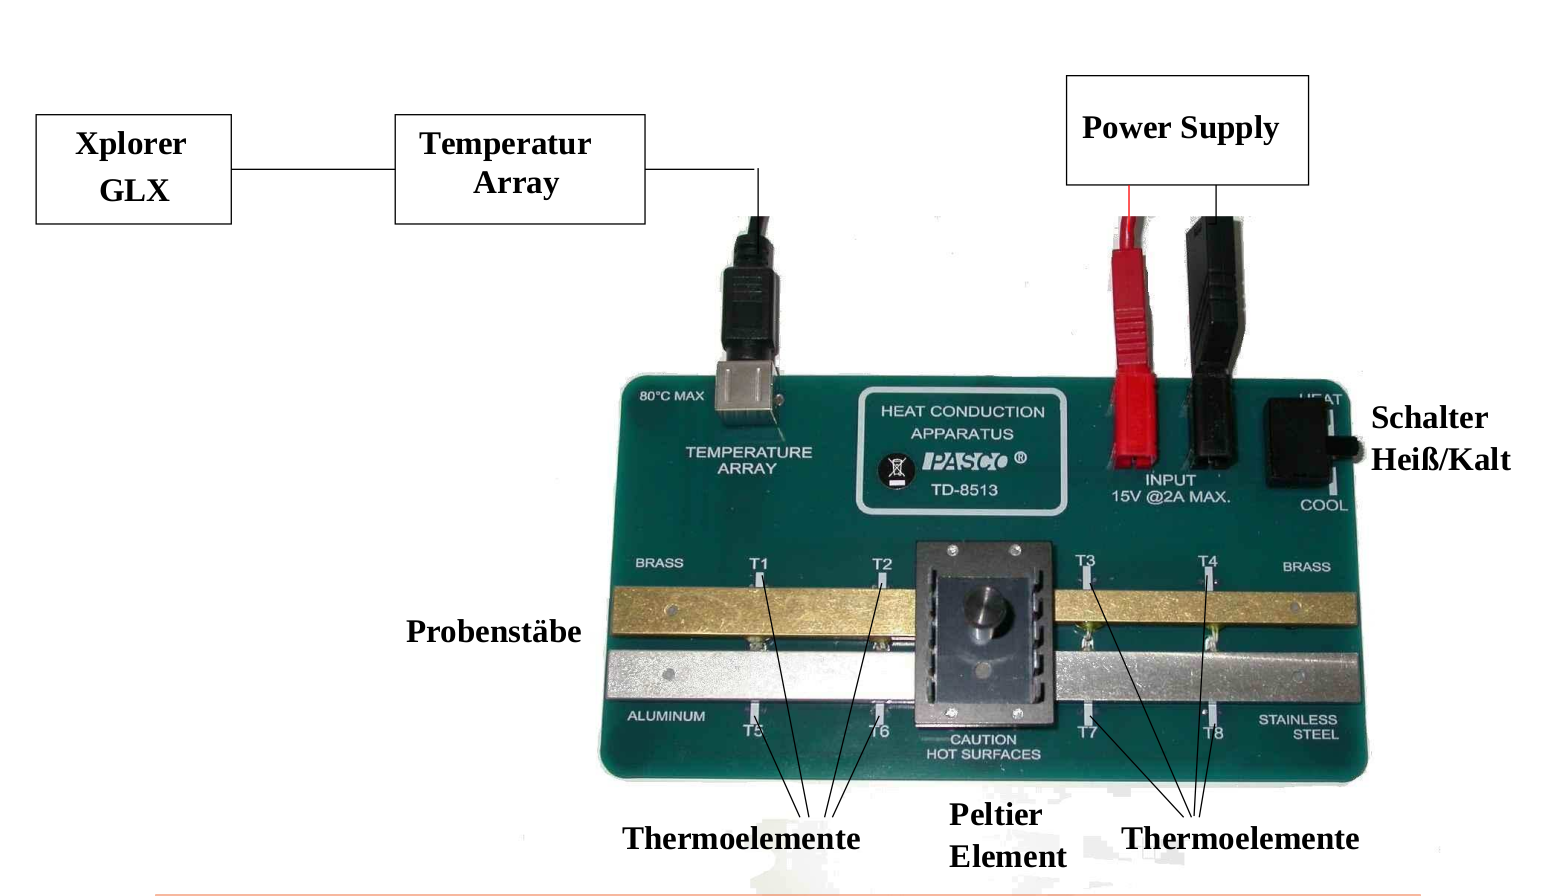
\includegraphics[height=7cm]{data/Bild2.png}
\caption{Versuchsaufbau auf der Grundplatte.}
\label{fig:aufbau}
\end{figure}


\begin{figure}
\centering
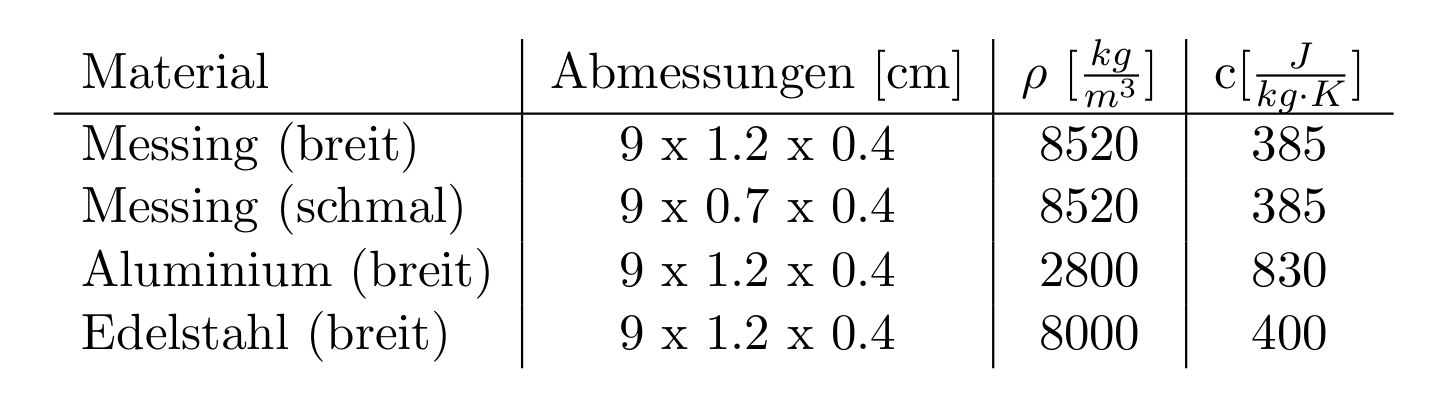
\includegraphics[height=4cm]{data/Bild1.png}
\caption{Daten der verwendeten Metallstäbe.}
\label{fig:daten}
\end{figure}

Der Versuchsaufbau ist in Abbildung \ref{fig:aufbau} dargestellt. Auf dieser Grundplatte befinden sich die vier Metallstäbe, welche auf ihre Wärmeleitfähigkeit untersucht werden sollen. Diese werden über ein Peltier-Element simultan erhitz und abgekühlt. In diesem Versuch werden zwei Messing-, ein Aluminium- und ein Edelstahlstab verwendet, dessen Abmessungen, Dichten und spezifische Wärmekapazitäten in Abbildung \ref{fig:daten} dargestellt sind. Über die acht Thermoelemente wird mit einem Datenlogger (Xplorer GLX) die jeweilge Temperatur gemessen. Eine Wärmeisolierung wird über die Stäbe gelegt, um die Umgebungswärme möglichst gut abzuschirmen.
Vor Beginn der Messungen werden alle Verkabelungen, der Aufbau und die Funktionalität des Datenloggers überprüft. Nach Abschluss jeder Messung wird die Isolierung entfernt und der Schalter auf "cool" gestellt,um den Abkühlungsvorgang zu beschleunigen. 


Zum bestimmen der Wärmeleitfähigkeit wird einmal die statische Methode und ein einmal eine dynamische Methode verwendet. In dem Versuch wird dazu für die dynamische Methode das Angström-Messverfahren verwendet.


\subsection{Statische Methode}
Bei der statischen Methode wird das Peltier-Element mit einer Betriebsspannung von $U_P=5\si{\volt}$ versorgt. Der Strom soll dabei maximal sein. Der Datenlogger wird auf eine Abtastrate von $\Delta t_{\text{GLX}}=5\si{\s}$ eingestellt. Daraufhin wird der Schalter auf "heat" gestellt. Die Stäbe werden solange erwärmt, bis das Thermoelement 7 ungefähr 45\textcelsius \,anzeigt. 
Nach Abkühlung, wenn die Temperaturen unter 30\textcelsius \,gesunken sind, wird die dynamische Methode durchgeführt.

\subsection{Angström-Messverfahren}
Die Betriebsspannung des Peltier-Elements wird auf $U_P=8\si{\volt}$ erhöht und die Abtastrate auf $\Delta t_{\text{GLX}}=2\si{\s}$ erniedrigt.
Im folgenden wird der Schalter, angefangen mit dem Erwärmungsvorgang, periodisch alle $40 \si{\s}$ umgeschaltet. So werden die Stäbe periodisch erwärmt und abgekühlt, sodass Temperaturwellen in ihnen entstehen können. Dieser Vorgang läuft über 6 Perioden, während durchgehend Messungen durch den Datenlogger vorgenommen werden.
Die Stäbe werden wieder bis auf eine Temperatur von ca. 30\textcelsius \,gekühlt.

Da Edelstahl eine geringe Wärmeleitfähigkeit besitz, und dadurch bei einer Periodendauer von $80\si{\s}$ keine gut verwertbaren Messungen vorgenommen werden können, wird die gleiche Methode erneut mit einer Periodendauer von $200\si{\s}$ durchgeführt.

Nach Beendigung der Messungen werden die Stäbe ein letztes Mal gekühlt.
%Was wurde gemessen bzw. welche Größen wurden variiert?